% ==============================================================================
% PG - Israel dos Santos Candeias
% Capítulo 2 - Referencial Teórico
% ====================================== 2.0 ================================
\chapter{Referencial Teórico e Tecnologias Utilizadas}
\label{sec-referencial}
% Este capítulo deve apresentar os aspectos relativos ao conteúdo teórico relevante para o trabalho.  Incluirá conhecimento adquirido a partir de livros, artigos, relatórios técnicos, dissertações, teses e outros materiais bibliográficos.  O capítulo deve apresentar, além do referencial teórico, informações sobre as tecnologias utilizadas no trabalho. O capítulo deve ter cerca de 12-15 páginas e deve demonstrar conhecimento básico da literatura técnico-científica sobre o tema abordado no trabalho.
Neste capítulo serão apresentados os conceitos teóricos que guiaram o desenvolvimento do jogo, bem como as tecnologias usadas para implementar o sistema, no capítulo \ref{sec-principios-de-design-de-software} abordamos alguns dos conceitos fundamentais de engenharia de software e também como isso foi usado nessa trabalho, na seção \ref{sec-desenvolvimento-de-jogos} é exposto alguns princípios básicos de desenvolvimento de jogos e as ferramentas e padrões que foram utilizadas na programação, a seção \ref{sec-mapas} fala sobre os programas que foram utilizados para o desenvolvimento de mapas desse jogo e a seção \ref{sec-pixel-art} explica como a parte artística do jogo foi feita e brevemente a ferramenta que foi utilizada.
% colocar os links para as seções explicando oq cada uma fala 

% =============================== 2.1 Princípios de Design de Software ===========================
\section{Princípios de Design de Software}
\label{sec-principios-de-design-de-software}
Os princípios de design de software constituem diretrizes fundamentais para o desenvolvimento de sistemas de software eficazes, robustos e manuteníveis. Esses princípios orientam todo o ciclo de vida do software desde o surgimento da ideia até o sistema em produção. 
\subsection{Engenharia de Software}
A engenharia de software é a área da computação que se preocupa em propor e aplicar princípios de engenharia na construção de softwares\cite{EngSoftMod} ou seja é uma área de estudos da computação que se preocupa em projetar, arquitetar melhorar a qualidade dos produtos de software aumentando assim a produtividade no processo de desenvolvimento. 

Para seguir as práticas recomendadas de engenharia de software o primeiro passo a ser definido é qual paradigmas de processo de software ser seguido, existem vários modelos para diferentes cenários possíveis, o escolhido para esse trabalho foi o modelo evolutivo.

O modelo evolutivo como o próprio nome sugere, os requisitos vão evoluindo conforme a aplicação evolui, esse processo ocorre em paralelo à evolução da aplicação, esse paradigma é muito útil quando o cliente não tem todas as funcionalidades necessárias para a solução. Nesse contexto foi oque mais se adequou a esse trabalho tendo em vista que nem todos os requisitos eram bem definidos de início e as funcionalidades do jogo precisam ser validadas frequentemente, uma vez que, a jogabilidade precisa ser atraente ao público, então a cada nova versão foram realizadas reuniões com colegas, e com a orientadora, a fim de receber feedbacks que auxiliem na melhoria dos recursos de modo contínuo.

A Figura \ref{spiral-model} ilustra esse modelo

\newpage
\begin{figure}
    \centering
    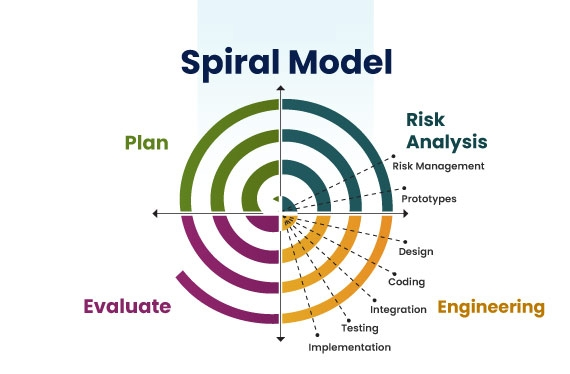
\includegraphics[width=0.9\linewidth]{figuras/spiral-model.jpg}
    \caption{Ciclo de vida do modelo espiral}
    \label{spiral-model}
\end{figure}
Cada uma das atividades realizadas no modelo ilustrado acima são:
\begin{itemize}
    \item \textbf{Planejamento:} A fase de planejamento é base sobre a qual todo o projeto de desenvolvimento de software deve ser construído. Durante essa fase foram definidos os requisitos e as ferramentas que seriam utilizadas;
    \item \textbf{Análise de riscos:} Nessa fase é feito tanto o levantamento dos riscos associados ao desenvolvimento do sistema, mas também como mitigá-los no geral sendo uma etapa para gerenciar os riscos, e na avaliação da viabilidade técnica;
    \item \textbf{Engenharia (Projeto e Codificação):} Aqui é onde são desenvolvidos os o designs do software, codificação, integração, testes e por fim a implantação no sistema;
    \item \textbf{Validação:} Ao chegar nessa fase já temos uma versão inicial do projeto, agora podemos coletar feedbacks o observações sobre o sistema, essa etapa é fundamental nessa abordagem, pois a qualidade da próxima versão é diretamente proporcional a qualidade dos feedbacks aqui coletados;
\end{itemize}

Essas Etapas se repetem num \textit{loop}, o número exato de \textit{loops} do modelo é indefinido e varia de projeto para projeto. Cada loop da espiral é nomeado fase do processo de desenvolvimento de software.

%  ================================ 2.2 Princípios de Game Design ================================
% 

% =================== PYGAME-CE =======================================
\section{Desenvolvimento de Jogos}
\label{sec-desenvolvimento-de-jogos}
Um jogo é um tipo de aplicativo utilizado não apenas para fins de entretenimento, mas também para objetivos mais sérios, com potencial de aplicação em diversos setores, como educação, negócios e saúde.
Desenvolver um jogo é uma tarefa desafiadora devido às diversas atividades multidisciplinares envolvidas, tornando o processo altamente complexo. A combinação de elementos como som, arte, sistemas de controle, inteligência artificial (IA) e fatores humanos confere ao desenvolvimento de jogos características distintas em relação ao desenvolvimento de software tradicional. 

\subsection{Princípios de Game Design}
Em um jogo com finalidade pedagógica, é essencial que tenha elementos a favor da diversão e do entretenimento é importante que o jogo esteja a favor do entretenimento, inclusive seus elementos educativos. Muitos jogos educacionais infringem este princípio por se preocuparem demais com as questões educacionais que os jogadores abandonam e jogo e o propósito do jogo não é alcançado, é necessário pensar se aquele elemento educacional vai contribuir com a diversão de fato. Para alcançar esse objetivo uma equipe de desenvolvimento de jogos.

Nos primeiros dias do desenvolvimento de videogames, os jogos eram
criados por grupos pequenos de pessoas, porém, com a complexidade dos jogos aumentando e a industria vendo oportunidades sérias, as equipes eventualmente foram acompanhando o ritmo a especialização está se tornando cada vez mais necessária à medida que os jogos se tornam maiores uma equipe de produção média inclui vários membros. Atualmente, uma equipe de desenvolvimento de jogos engloba profissionais multidisciplinares de diversas áreas, cada um com um foco especifico para a produção do jogo. Scott Rogers cita em seu livro \cite{GameDesign} as seguintes: 
\begin{itemize}
    \item \textbf{Programador(a):} Responsável pela programação do software do jogo e das ferramentas utilizadas quando se aplicam também escreve o documento técnico;
    \item \textbf{Artista:} Responsável pela representação visual dos componentes do jogo desde as interfaces aos personagens estipulados no documento técnico ;
    \item \textbf{Designer do Jogo:} cria as ideias e regras que compõem o jogo do conceito até a forma final também cuida da documentação do sistema de interação;
    \item \textbf{Produtor(a): }Responsável por supervisionar toda a equipe de desenvolvimento do jogo;
    \item \textbf{Testador:} Responsável por jogar compulsivamente o jogo e relatar problemas ou \textit{bugs} encontrados
    \item \textbf{Compositor:} Aquele responsável por criar temas e tilhas marcantes que sejam capazes de compor o cenário do jogo e passar os sentimentos que o designer do jogo estipulou.
    \item \textbf{Designer de Som:} cria todos os efeitos sonoros que são usados em um jogo;
    \item \textbf{Roteirista:}  Responsável por escrever o manual do jogo e qualquer material de suporte fictício, como  biografias de personagens;
    \item \textbf{Gerente de produto:} Um gerente de produto trabalha com a equipe de desenvolvimento e os gerencia com base no cronograma de produção;
    \item \textbf{Diretor Criativo:} é responsável por toda a gestão criativa de uma marca ou projeto;
    \item \textbf{Diretor(a) de Arte:} Responsável por ajudar a equipe a criar um estilo visual do jogo e trabalham com as equipes de marketing a fim de criar os designs dos produtos;
    \item \textbf{Diretor(a) Técnico:} Eles revisam e recomendam ferramentas e softwares para equipes para ajudá-las a trabalhar de forma mais eficiente. Eles fornecem suporte técnico e aconselhamento quando há deficiências na equipe;
\end{itemize}

\subsection{Pygame-ce}
Pygame-ce (Community Edition) \footnote{https://github.com/pygame-community/pygame-ce/} é uma biblioteca multiplataforma gratuita e de código aberto que surgiu de um fork do projeto pygame por seus antigos desenvolvedores principais, ela foi criado após desafios impossíveis os impedirem de continuar o desenvolvimento upstream. Seu foco é construir aplicativos multimídia como videogames utilizando a linguagem Python. Ela está sobre a licença GNU LGPL version 2.1 oque significa que pode ser usada em qualquer projeto que quiser, mas se forem feitas quaisquer alterações ou adições ao codigo-fonte, elas devem ser lançadas com uma licença compatível. 
 Ela usa a biblioteca SDL (Simple DirectMedia Layer)\footnote{SDL (Simple DirectMedia Layer) \url{https://www.libsdl.org/}} que é uma biblioteca de desenvolvimento multiplataforma também de código aberto e escrita em C, projetada para fornecer acesso de baixo nível a hardware de áudio, teclado, mouse, joystick e gráficos via OpenGL e Direct3D além de várias outras bibliotecas populares para abstrair as funções mais comuns. O SDL age como um \textit{wrapper} de camada fina e multiplataforma, fornecendo suporte a operações de pixel 2D, som, acesso à arquivos, manipulação de eventos, temporizadores, threading,
As principais funcionalidades do pygame incluem
\begin{itemize}
    \item carregar e exibir imagens;
    \item criar animações e renderizar quadros de jogos;
    \item adicionar música de fundo e efeitos sonoros;
    \item Manipulação de dispositivos de entrada;
    \item Gerenciamento de sprites através de classes integradas;
\end{itemize}

Como a maioria das bibliotecas no python ela pode ser adicionada via \textit{prompt} de comandos do sistema operacional  por meio do pip\footnote{pip \url{https://pip.pypa.io/en/stable/}}, o pip é um sistema de gerenciamento de pacotes para Python, usado para instalar e gerenciar pacotes de software escritos na linguagem de programação Python. Ele simplifica o processo de instalação, atualização e remoção de pacotes Python e suas dependências, as listagens seguintes mostram como é feito o processo de instalação e um programa inicial \footnote{Pygame Docs \url{https://pyga.me/docs/}}. 

\newpage
\begin{lstlisting}[language=bash,breaklines, caption= Instalação Pygame]
pip install pygame-ce
\end{lstlisting}
\lstinputlisting[label=lst-circle-movement, caption=Exemplo de código Pygame Para Mover um Circulo., language=Python, float=htpb]{codigos/circle_movement.py}
% completar aqui
Esse é um exemplo básico de um programa pygame com um circulo que se move, na linha (2) importamos o pygame e dizemos ao compilador para carregar os seus módulos, nas linhas (5) à (8) fazemos a inicialização básica de todo código pygame onde inicializamos o pygame configuramos a tela inicial, configuramos as variáveis de controle \textit{clock} e \textit{running}, a linha (11) é definido a posição inicial do círculo, na linha (13) é onde começa o \textit{loop} principal do jogo que consistem em:
\begin{enumerate}
    \item verificar se o jogador fechou o jogo (linhas 16 a 18);
    \item preencher toda a tela com a cor roxa (linha 21);
    \item desenhar o círculo vermelho na posição \textit{player\_pos} (linha 23);
    \item fazer a captura da entrada do jogador (25) e se for o alguma das ("w", "s", "a", "d") move o círculo a respectiva direção (linhas 26 a 33);
    \item a linha (36) atualiza o conteúdo de toda essa exibição;
    \item e por fim (linha 41) essa variável;
\end{enumerate}

\subsection{Game Loop}
Jogos eletrônicos e programas interface gráfica não dependem da entrada do usuário para continuar funcionando, mesmo se nada for feito, o jogo ainda deve ser constantemente atualizado. Isso caracteriza um \textit{game loop} ou \textit{event loop}, independentemente da \textit{input} do jogador, a aplicação continuará sendo executado.
Um game loop deve ter necessariamente três elementos (i)input onde é feito o gerenciamento da entrada de controles do jogador, que pode ser o mouse, teclado \textit{joystick} e afins (ii)update, neste método são realizadas todas as atualizações que são impostas a função, desde a movimentação de personagens, a checagem de transições, ou a morte do jogador por exemplo (iii)render essa função é responsável por renderizar, ou seja desenhar todos os sprites na tela de acordo com a ordem que é definida na programação.
\begin{figure}[h!]
    \centering
    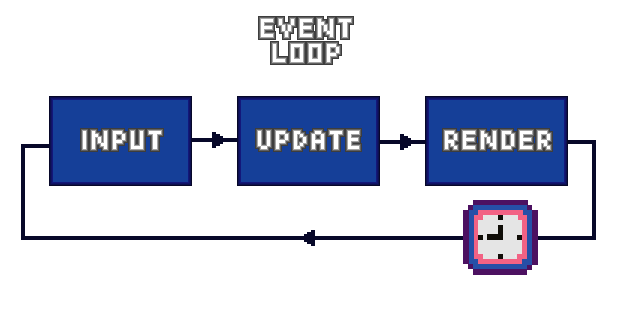
\includegraphics[width=1\linewidth]{figuras/event-loop.png}
    \caption{Event Loop}
    \label{fig:event-loopl}
\end{figure}

% Delta time
\subsection{Delta Time}
 \textit{Delta time} ou diferença de tempo é uma variável de controle que tem um valor numérico armazenado nela, esse valor corresponde a diferença de valores do ultimo \textit{clock} e o clock atual.
 \begin{equation}
    \Delta t = t' - t
    \label{eq:dt_equation}
\end{equation}

 Quando dizemos que um jogo roda a 30 quadros por segundo, temos o valor do delta é \(\frac{1}{30}\) isso significa também dizer que o game loop do jogo leva \(\frac{1}{30}\) segundos para ser executado, isso é utilizado para resolver o problema a evolução dos computadores criou, onde se tinha jogos feitos para máquinas quem tinham recursos escassos, e se um computador atual executasse um jogo dos anos 80 hoje sem nenhum mecanismo de controle, o jogo rodaria a alguns milhares de quadros e a experiência não seria boa se não fosse utilizado desse \textit{pattern} de jogos, não existiria uma normalidade entre dispositivos.


% coisas para explicar?
% colocar um codigo com \href{https://pyga.me/docs/ref/music.html}{pygame.mixer.música} \href{https://pyga.me/docs/ref/draw.html}{pygame.draw} 
% \href{https://pyga.me/docs/ref/event.html}{pygame.event} 
% \href{https://pyga.me/docs/ref/font.html}{pygame.font} 
% \href{https://pyga.me/docs/ref/image.html}{pygame.image} 
% \href{https://pyga.me/docs/ref/key.html}{pygame.key} 
% \href{https://pyga.me/docs/ref/rect.html}{pygame.Rect} 
% \href{https://pyga.me/docs/ref/sprite.html}{pygame.sprite} 
% \href{https://pyga.me/docs/ref/surface.html}{pygame.Surface} 
% \href{https://pyga.me/docs/ref/transform.html}{pygame.transform} 
% \href{https://pyga.me/docs/ref/window.html}{pygame.Window} 
% completar aqui

%  ======================================= 2.3 Mapas =================================
\section{Mapas}
\label{sec-mapas}
% explicar oq e um editor de mapas

A maioria dos jogos tem seus cenários, esses ambientes são de suma importância pois são neles onde os jogadores passam a maior parte do tempo, eles não são desenhados de forma totalmente manual, são utilizadas ferramentas que auxiliam na sua criação, são os softwares editores de mapas.

Um Editor de mapas é uma ferramenta que ajuda os designers e desenvolvedores do jogos a criarem de forma visual e intuitiva os mapas dos seus jogos, praticamente todos os jogos usam uma ferramenta para esse propósito e existem editores 2D quanto 3D para essa finalidade, em 2D existe uma técnica denominada \textit{Tile-Based} essa técnica de desenvolvimento de jogos eletrônico onde o cenário é feito por pequenas imagens quadradas, retangulares ou hexagonais chamados \textit{tiles} (ladrilhos).
% citar jogos populares que utilizam essa técnica (dofus)

\subsection{Tiles e Tilesets}
Tilesets são coleções de pequenas imagens reutilizáveis chamados “tiles” organizadas em uma grade. Cada tile representa uma pequena parte do mundo do jogo. Um tile pode representar um pedaço de chão, um segmento de uma parede ou uma decoração. Ao combinar diferentes tiles em diferentes posições temos um cenário que pode ser utilizado como fase de um jogo é um recurso gráfico para desenhar níveis e outros componentes estáticos do seu jogo de forma rápida e eficiente, já que não é necessário desenhar toda a área jogável.
Na figura \ref{fig:tileset-orthogonal} temos um exemplo de tileset ortogonal para um jogo a câmera vista de cima, e \ref{fig:tileset-platform-orthghonal} ilustra um tileset ortogonal para jogos plataforma.
\begin{figure}[h!]
    \centering
    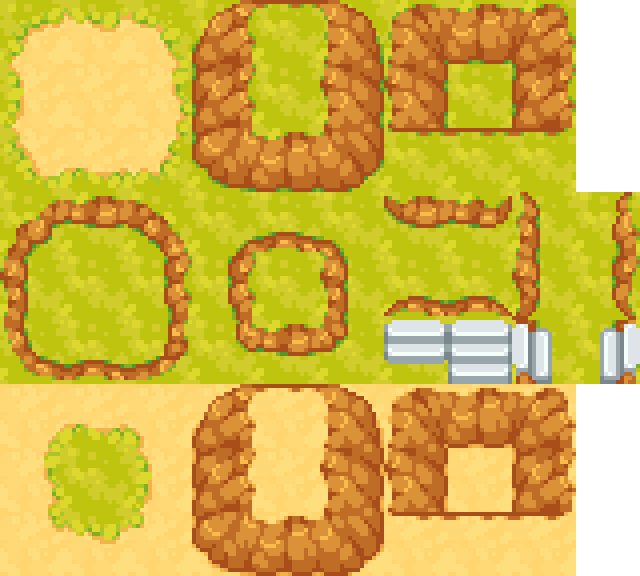
\includegraphics[width=0.5\linewidth]{figuras/tileset.png}
    \caption{Exemplo de Tileset Ortogonal}
    \label{fig:tileset-orthogonal}
\end{figure}
\begin{figure}[h!]
    \centering
    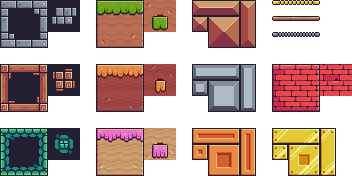
\includegraphics[width=0.5\linewidth]{figuras/tileset-orthogonal-platform.png}
    \caption{Exemplo de Tileset Ortogonal Para Jogos De Plataforma}
    \label{fig:tileset-platform-orthogonal}
\end{figure}

\subsection{Tiled}
O Tiled \footnote{Tiled Map Editor \url{https://www.mapeditor.org}} é um editor de níveis 2D que ajuda game designers a desenvolverem o conteúdo de seus jogos. Seu recurso principal é editar mapas de tiles de várias formas, mas ele também suporta posicionamento de imagens livre, bem como maneiras eficientes de colocar metadados em seus sprites que futuramente poderão serem usados pela programação.
Camada de blocos

Ele suporta camadas de tiles retangulares retas e também camadas isométricas projetadas, isométricas escalonadas e hexagonais escalonadas. Um tileset pode ser uma única imagem contendo muitos tiles ou pode ser uma coleção de imagens individuais. Também é capaz de suportar algumas técnicas de simulação de profundidade através de deslocamento de camadas e alteração da ordem de renderização dos componentes.

O Tiled também suporta camadas de objetos, que podem ser usadas para colocar imagens, também é possível adicionar objetos como retângulos, pontos, elipses, polígonos, polilinhas e ladrilhos. O posicionamento de objetos não se limita à grade de ladrilhos e os objetos também podem ser dimensionados ou girados. As camadas de objetos oferecem muita flexibilidade para adicionar quase qualquer informação ao seu nível que seu jogo precise.
Na Figura \ref{fig:map-creation} temos a configuração inicial da criação de um mapa.
\begin{figure}[h!]
    \centering
    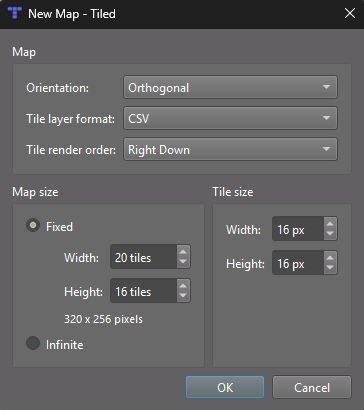
\includegraphics[width=0.5\linewidth]{figuras/new-map-tiled.png}
    \caption{Criação de mapa}
    \label{fig:map-creation}
\end{figure}

As características mais importantes a serem destacadas nessa tela são:
\begin{itemize}
    \item \textbf{Orientação (Orientation):} A orientação define como é o estilo de visualização do seu jogo, sendo possíveis 4 estilos “ortogonal”, “isométrico”, “escalonado” e “hexagonal”;
    \item \textbf{Tamanho do mapa \textit{(Map Size}):} nessa parte é definido o tamanho do mapa, é possível alterar os valores no decorrer da criação, o próprio software faz o calculo de quantos pixels o mapa ficará, na figura cada tile tem 32 píxels de tamanho, e o mapa é um quadrado 10 x 10 , sendo assim o tamanho final do mapa é 320 x 320
    \item \textbf{Tamanho do tile \textit{(Tile Size)}:}, essa é a informação mais importante dessa página, é nessa opção que se define o tamanho do tile que vai ser representado na tela, isso significa que cada azulejo do mapa terá exatamente esse tamanho, quando for a  hora de importar o tileset para o programa é importante garantir que o  tileset tem o mesmo tamanho do tile do mapa.
\end{itemize}
Com o mapa em branco criado agora é necessário importar um tileset para começar a desenhar o mapa a figura \ref{fig:new-tileset}  ilustra esse processo.
\begin{figure}[h!]
    \centering
    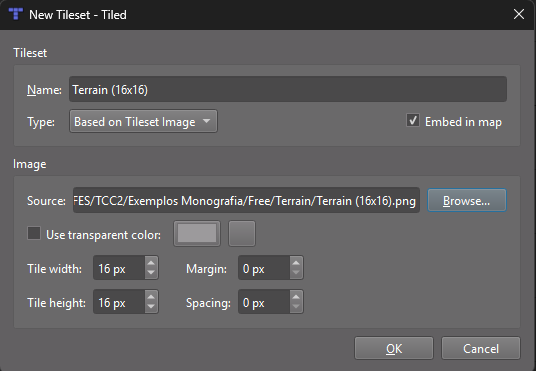
\includegraphics[width=0.5\linewidth]{figuras/new-tileset.png}
    \caption{Enter Caption}
    \label{fig:new-tileset}
\end{figure}
As Informações mais importantes aqui são:
\begin{itemize}
    \item \textbf{Procurar \textit{(Browse)}:} nessa opção você vai carregar o arquivo para o programa;
    \item \textbf{Tipo \textit{(Type)}:} aqui dizemos ao programa se é uma imagem única com múltiplos tilesets, ou uma imagem unica;
    \item \textbf{Largura do Tile e Altura do tile \textit{(Tile Width)} \textit{(Tile Height)}:} Nessa parte você está dizendo ao programa como "fatiar" a imagem que está recebendo, dividindo assim em vários azulejos únicos reutilizáveis, com essas configurações ficamos com um algo assim;
    \begin{figure}[h!]
        \centering
        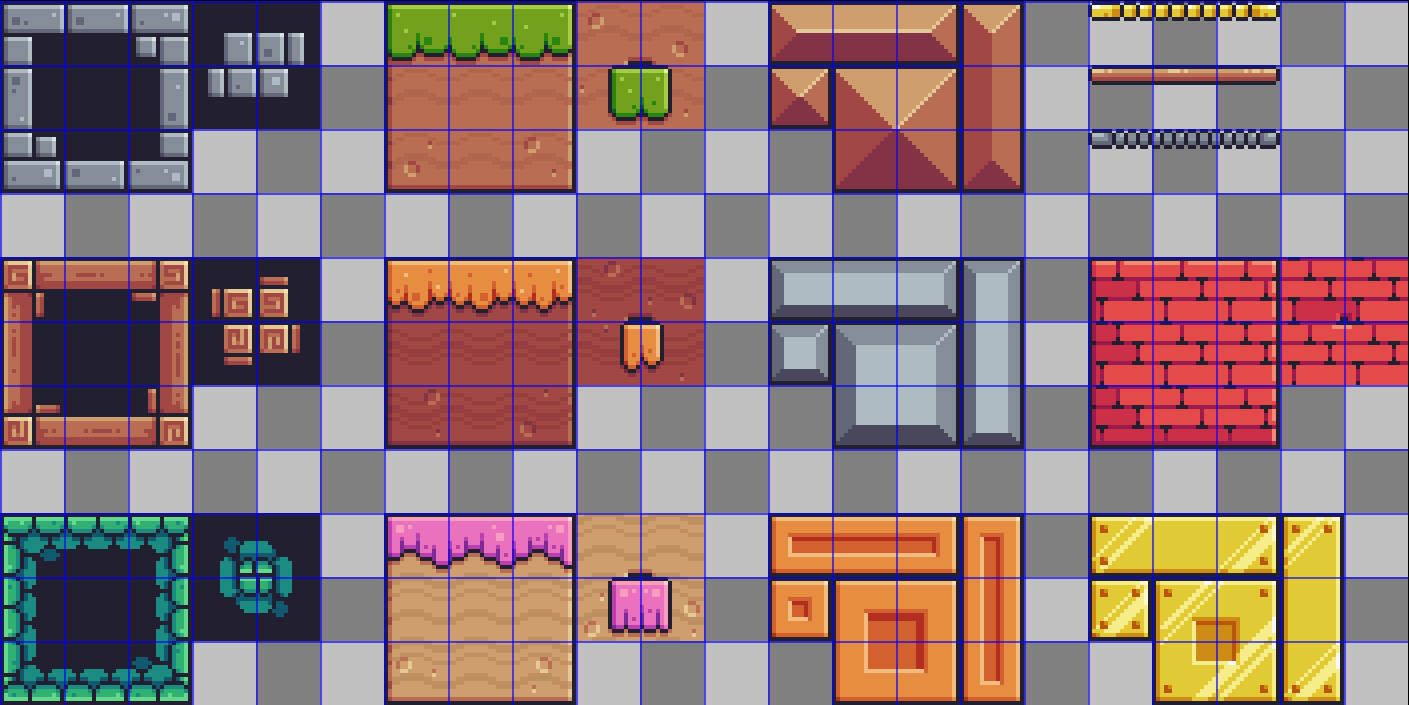
\includegraphics[width=0.8\linewidth]{figuras/tileset-dividido.png}
        \caption{Tileset dividido}
        \label{fig:tileset-dividido}
    \end{figure}
\end{itemize}

\subsection{Camadas}
Antes de começar a desenhar nossos cenários é importante já ter definido de antemão quais serão as camadas utilizadas no projeto, para evitar o trabalho de ficar movendo objetos e tiles de uma camada a outra. Camadas ou \textit{layers} no tiled funcina definindo a ordem em que as coisas serão desenhadas na tela, de forma \textit{bottom-up} ou seja, os tiles serão renderizados de baixo para cima, onde, se tiver blocos sobrepostos, o que está mais acima tem prioridade. A figura \ref{fig:layers} mostra um mapa que tem quatro camadas, (i) terreno, (ii) topo do terreno (iii) objetos e (iv) entidades. 
\begin{figure}[h!]
    \centering
    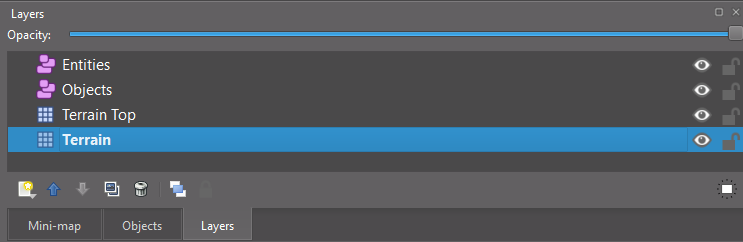
\includegraphics[width=1\linewidth]{figuras/layers.png}
    \caption{Camadas no Tiled}
    \label{fig:layers}
\end{figure}


Existem 4 tipos de camadas no Tiled sendo duas delas as utilizadas nesse trabalho  \textbf{(i) Camada de tiles}, é nela que é feita os terrenos do jogo bem como as coisas acima do terreno sem colisão (na figura \ref{fig:layers} as camadas "\textit{Terrain}" e "\textit{Terrain} Top", \textbf{(ii) camada de objetos} (Camadas "\textit{Entities}" e "\textit{Objects}" da figura
\ref{fig:layers} essa camada é muito útil pois o software permite adicionar metadados, dados com chave/valor aos dados presentes aqui, a figura \ref{fig:add-custom-property-object} exemplifica como adicionar uma propriedade "quebrável" a uma caixa.
\begin{figure}[h!]
    \caption{Adicionando uma propriedade personalizada a um objeto}
    \label{fig:add-custom-property-object}
    \subfloat{
        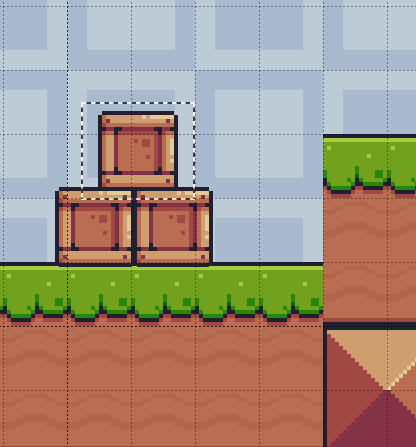
\includegraphics[width=0.35\linewidth]{figuras/example-map.png}
    }\hfill
    \subfloat{
        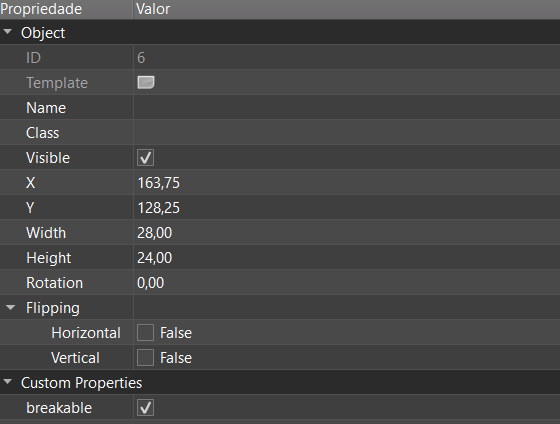
\includegraphics[width=0.5\linewidth]{figuras/custom-property.png}
    }
\end{figure}
Ao salvar essas configurações o programa gera um arquivo com a extensão '.tmx' que é o acrônimo de Translation Memory eXchange, é um formato baseado no 'xml' devido a isso faz o uso de tags e atributos de arquivo padrão usado na indústria de tradução para armazenar e trocar memórias de tradução, basicamente consiste em uma seção de cabeçalho, seguido por uma ou várias seções de corpo, cada uma contendo unidades de tradução. A listagem a seguir ilustra isso.

\newpage
\begin{lstlisting}[language=xml,breaklines, caption= example.tmx terrain layer]
<?xml version="1.0" encoding="UTF-8"?>
<map version="1.10" tiledversion="1.11.0" orientation="orthogonal" renderorder="right-down" width="20" height="16" 
tilewidth="16" tileheight="16" infinite="0" nextlayerid="5" nextobjectid="7">
 <tileset firstgid="1" name="Terrain (16x16)" tilewidth="16" tileheight="16" tilecount="242" columns="22">
  <image source="Free/Terrain/Terrain (16x16).png" width="352" height="176"/>
 </tileset>
 <tileset firstgid="243" name="images" tilewidth="28" tileheight="24" tilecount="1" columns="0">
  <grid orientation="orthogonal" width="1" height="1"/>
  <tile id="0">
   <image source="Free/Items/Boxes/Box1/Idle.png" width="28" height="24"/>
  </tile>
 </tileset>
 <tileset firstgid="244" name="Blue" tilewidth="16" tileheight="16" tilecount="16" columns="4">
  <image source="Free/Background/Blue.png" width="64" height="64"/>
 </tileset>
 <layer id="1" name="Terrain" width="20" height="16">
\end{lstlisting}

\begin{lstlisting}[language=xml,breaklines, caption= example.tmx object layer]
 <objectgroup id="3" name="Objects">
  <object id="4" gid="243" x="153" y="147.25" width="28" height="24"/>
  <object id="5" gid="243" x="172.5" y="147.25" width="28" height="24"/>
  <object id="6" gid="243" x="163.75" y="128.25" width="28" height="24">
   <properties>
    <property name="breakable" type="bool" value="true"/>
   </properties>
  </object>
 </objectgroup>
\end{lstlisting}


%  ======================================= PyTMX =======================================
\subsection{PyTMX}
% completar aqui
PyTMX\footnote{PyTMX \url{https://pytmx.readthedocs.io/en/latest/}} é um carregador de mapas para python/pygame projetado para jogos. Ele fornece carregamento inteligente de tiles com uma base de armazenamento rápida e eficiente. Ele manipula corretamente a maioria dos tipos de objetos Tiled, e também carrega metadados para eles, para que você possa modificar seus mapas e objetos no Tiled, em vez de modificar seu código-fonte ele inclui suporte completo para leitura desses dados para que possa definir parâmetros para coisas no Tiled, em vez de manter arquivos de dados externos, ou mesmo valores na fonte. Pytmx também é uma biblioteca e pode ser instalada por linha de comando com o pip, como exemplificado a seguir.
\begin{lstlisting}[language=bash,breaklines, caption= Instalação Pytmx]
pip install pytmx
\end{lstlisting}

\begin{lstlisting}[language=python,breaklines, caption= Uso Básico Pytmx]
import pytmx

tmxdata = pytmx.TiledMap("example.tmx")

print(tmxdata.width)
print(tmxdata.height)
print(tmxdata.tilewidth)
print(tmxdata.orientation)
print(tmxdata.layernames)
\end{lstlisting}

\begin{lstlisting}[language=bash,breaklines, caption= Saída]
>>> 20
>>> 16
>>> 16
>>> orthogonal
>>> {'Terrain': <TiledTileLayer[1]: "Terrain">, 'Terrain Top': <TiledTileLayer[2]: "Terrain Top">, 'Objects': <TiledObjectGroup[3]: "Objects">, 'Entities': <TiledObjectGroup[4]: "Entities">}
\end{lstlisting}

Para podermos usar esse mapa é necessário anteriormente importarmos ele para dentro do código isso é feito na linha 1, na linha 3 criamos uma variável para armazenar o mapa, e com isso temos acesso as informações presentes naquele mapa.

Agora para termos acesso aos metadados presentes na camada de objetos, por exemplo, podemos fazer uma iteração e verificação do nome do \textit{layer} com isso temos acesso aos objetos quebráveis.
\begin{lstlisting}[language=python,breaklines, caption= Verificação de Objetos Quebráveis]
for layer in tmxdata.visible_layers:
    if layer.name == 'Objects':
        for obj in layer:
            print(obj.properties['breakable'], obj.x, obj.y)
\end{lstlisting}

\begin{lstlisting}[language=bash,breaklines, caption= Saída]
>>> True 163.75 104.25
>>> True 152.25 123.0
>>> True 172.5 123.25
\end{lstlisting}










%  ======================================= Pixel Art ===================================
\section{Pixel Art}
\label{sec-pixel-art}
Pixel originada de (picture e element), ou seja, elemento de imagem sendo pix a abreviatura em inglês para pictures, é a menor unidade de uma imagem que e possível ser expressa digitalmente, se você fizer uma aproximação de uma foto digital ou de uma tela de celular, verá uma série de quadradinhos. Cada um deles é um pixel. A Pixel Art é um tipo de arte que usa pixels visíveis para compor uma imagem ou um vídeo, a junção de diversos pontos digitais de somado a criatividade e horas de dedicação proporciona obras de arte e animações que a ente humana não consegue acompanhar.

Em um monitor que permite imagens coloridas, cada pixel é composto por um conjunto de 3 pontos: vermelho, verde e azul. Nos melhores monitores, cada um desses pontos é capaz de exibir 256 tonalidades diferentes (o equivalente a 8 bits) com  a combinação dessas tonalidades dos três pontos é então possível exibir pouco mais de 16.7 milhões de cores diferentes (exatamente 16.777.216)  256 x 256 x 256, A quantidade de pixels a serem mostradas na tela depende do tamanho do display, por exemplo, em uma resolução HD (1280 x 720) temos 921.600 pixels, numa resolução 8K (7680 x 4320) temos 33.177.600 a serem preenchidos.

A pixel art surgiu nos anos 70 mas foi formalizada nos anos 80 nessa época era o início dessas tecnologia, os monitores ainda não possuíam a quantidade de pixels que temos atualmente. desenhar objetos na tela com "quadradinhos" era a única forma uma vez que era o único recurso que tinha na época mas que até nos dias atuais de forma despretensiosa é um estilo de arte que milhares de pessoas adoram 
nas figuras \ref{fig:mario} e \ref{fig:mega_man} vemos alguns exemplos de Pixel arts.
\begin{figure}[ht!]
    \caption{Exemplos de diferentes pixel arts em suas gerações esquerda Super Mario 8-bits (NES) /  Mega Man x4 32-bits (Playstation 1)}
    \label{fig:comparative-8bit-32-bit-pixel-art}
    \subfloat\label{fig:mario}1985.{
        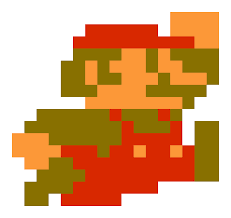
\includegraphics[width=0.35\linewidth]{figuras/mario-sprite-nes.png}
    }\hfill
    \subfloat\label{fig:mega_man}1998{
        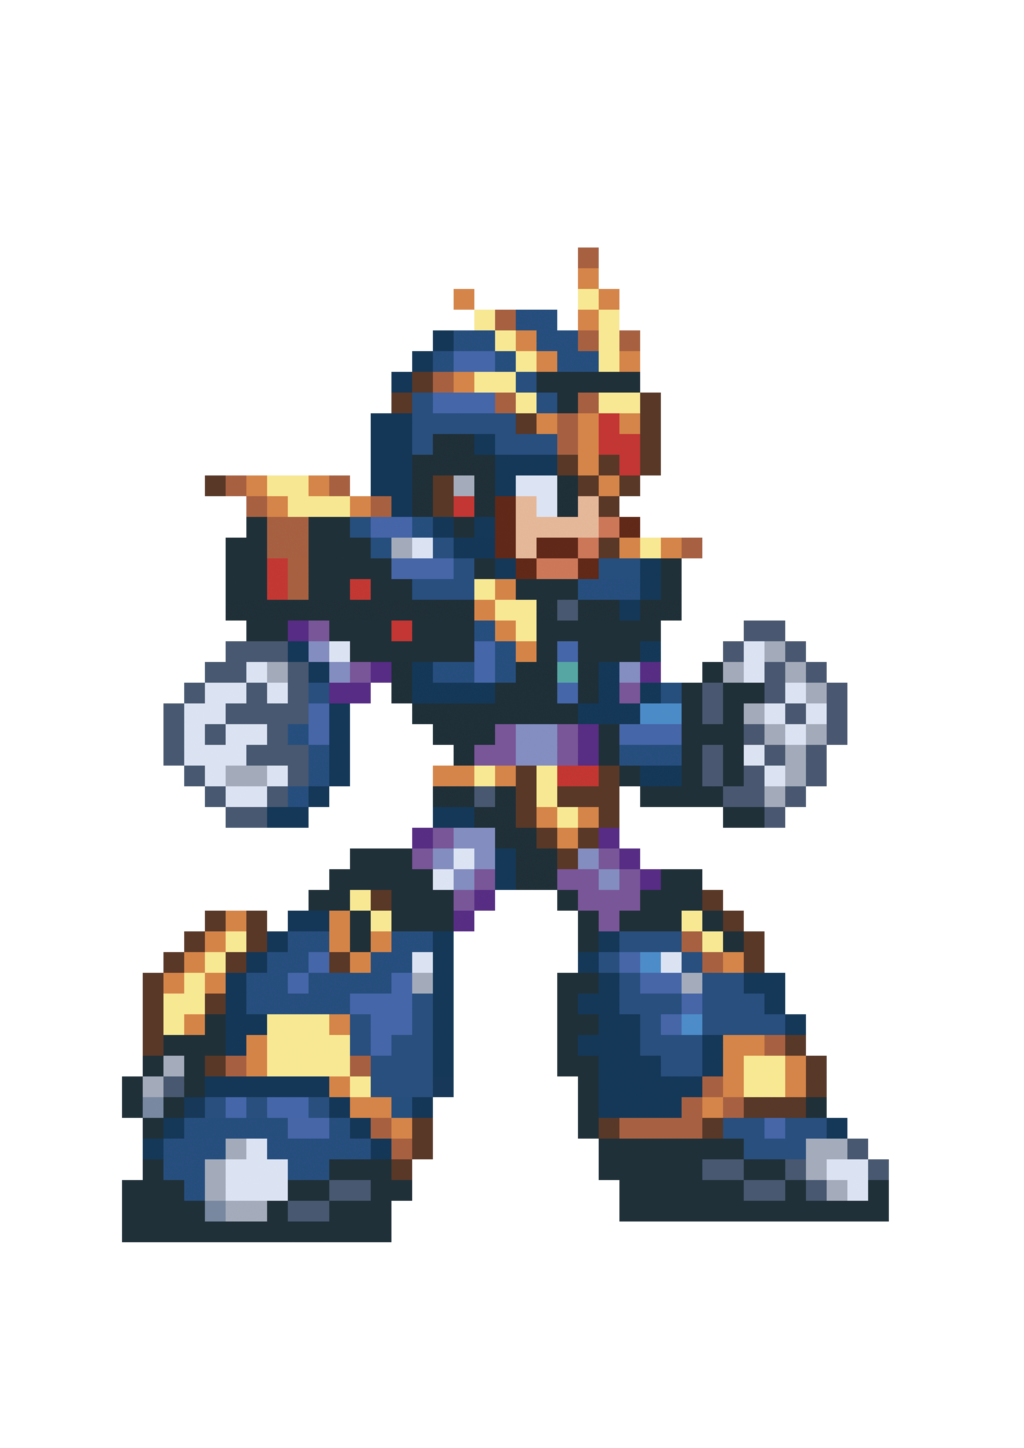
\includegraphics[width=0.3\linewidth]{figuras/mega-man-ps1.png}
    }
\end{figure}

\newpage
\subsection{Aseprite}  
% Para fazer um jogo é necessário ter sprites 
O Aseprite\footnote{Aseprite \url{https://www.aseprite.org}} é um software comercial especializado em pixel art, ele conta com recursos e ferramentas específicas para essa finalidade permitindo assim a criação de animações 2D para videogames. De sprites a pixel-art, gráficos estilo retrô a figura \ref{fig:aseprite} ilustra a tela básica do programa, a primeira vista ele é similar a outros programas de criação de imagens com exceção da grade quadriculada.  
\begin{figure}[ht!]
    \centering
    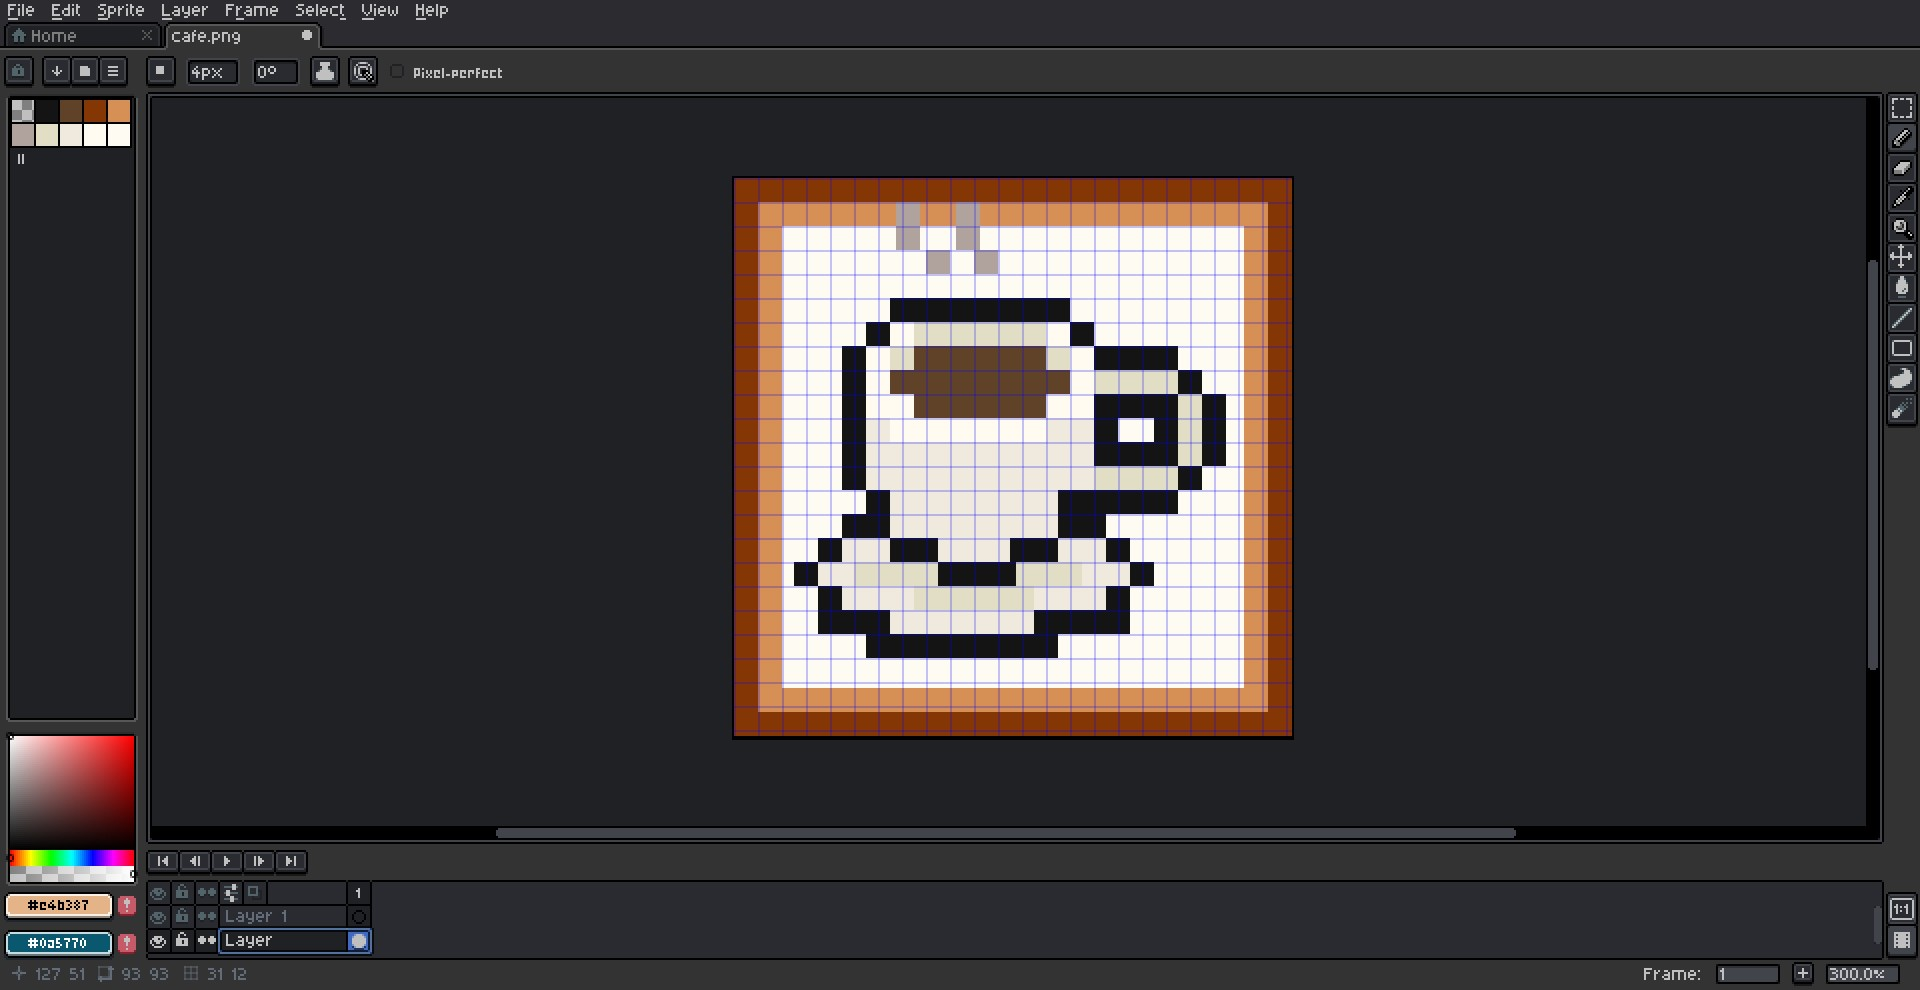
\includegraphics[width=1\linewidth]{figuras/aseprite.jpg}
    \caption{Visão Básica Aseprite}
    \label{fig:aseprite}
\end{figure}

Um Sprite é um objeto gráfico bidimensional (2D) usado em computação gráfica e particularmente em videogames. Ele normalmente consiste em uma imagem de bitmap ou uma série de imagens que são combinadas para criar uma animação. Um sprite pode ser pensado como uma entidade separada que existe dentro de uma cena maior, como um mundo de videogame. No Aseprite, um sprite consiste de uma sequência de quadros somados uma pilha de camadas. A intersecção de quadros e camadas cria uma matriz de células gráficas editáveis com imagens/pixels que podem ser editados com o editor de sprites . Camadas, quadros e células são visíveis na linha do tempo
\begin{figure}[h!]
    \centering
    
\includegraphics[width=1\linewidth]{figuras/sprite-frog.png}
    \caption{Ninja Frog Sprite de Pulo}
    \label{fig:enter-label}
\end{figure}
\subsection{Animação}
 A animação é a ilusão de movimento que nossos cérebros nos enganam para perceber quando vemos vários quadros estáticos de obras de arte reproduzidos em rápida sucessão.
Um quadro é uma única imagem estática em um sprite, se adicionarmos e alterarmos os quadros a uma certa velocidade, cria-se a a impressão de movimento, essa impressão é chamada animação. 
Em programação existem varias formas de fazer a animação uma delas é através de vetores, a técnica consiste em carregar uma imagem e dizemos ao computador que queremos dividir essa imagem e armazena-lo num vetor, a figura \ref{fig:sprite-animation} exemplifica isso, nesse caso um vetor de duas linhas e cinco colunas, assim para fazer a animação desse personagem, basta percorrer as imagens alternadamente enquanto capturamos a entrada do jogador e vemos se é movimento

\begin{figure}[h!]
    \centering
    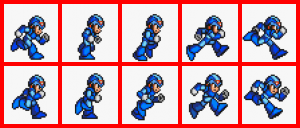
\includegraphics[width=0.8\linewidth]{figuras/megaman-sprite-animation-export.png}
    \caption{Sprite Animation}
    \label{fig:sprite-animation}
\end{figure}






